\documentclass{standalone}
\usepackage{amsmath, amsfonts, amsthm}
\usepackage{siunitx}
\usepackage{graphicx}
\usepackage{tikz}
\usepackage{circuitikz}
\usetikzlibrary{patterns}
\usepackage{scalerel}
\usepackage{pict2e}
\usepackage{tkz-euclide}
\usetikzlibrary{calc}
\usetikzlibrary{arrows.meta}
\usetikzlibrary{shadows}
\usetikzlibrary{external}
\usetikzlibrary{decorations.pathmorphing}
\usetikzlibrary{shapes.geometric}
\usetikzlibrary{arrows,shapes.gates.logic.US,shapes.gates.logic.IEC,calc}
\usepackage{pgfplots}
\pgfplotsset{compat=newest}
\usepgfplotslibrary{statistics}
\usepgfplotslibrary{fillbetween}

\begin{document}
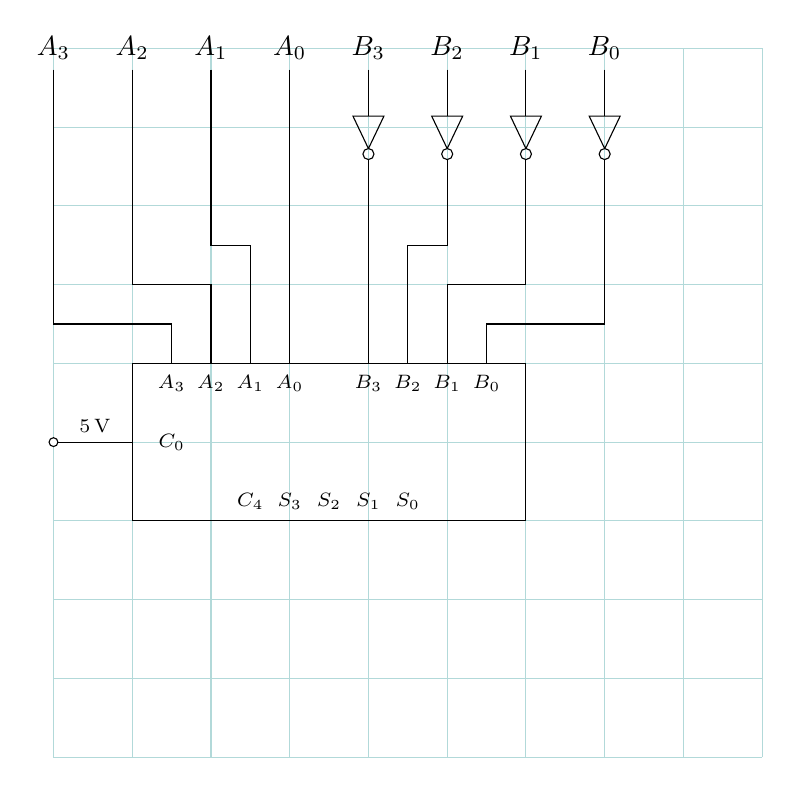
\begin{tikzpicture}
	\draw [help lines] (0,0) grid (9,-9);

	\node (A3) at (0,0) {$A_3$};
	\node (A2) [right of=A3] {$A_2$};
	\node (A1) [right of=A2] {$A_1$};
	\node (A0) [right of=A1] {$A_0$};

	\node (B3) [right of=A0] {$B_3$};
	\node (B2) [right of=B3] {$B_2$};
	\node (B1) [right of=B2] {$B_1$};
	\node (B0) [right of=B1] {$B_0$};

	\node ('B3) [not gate US, draw, rotate=-90] at (4,-1) {};
	\node ('B2) [not gate US, draw, rotate=-90, above of='B3] {};
	\node ('B1) [not gate US, draw, rotate=-90, above of='B2] {};
	\node ('B0) [not gate US, draw, rotate=-90, above of='B1] {};

	\draw (B3) -- ('B3.input);
	\draw (B2) -- ('B2.input);
	\draw (B1) -- ('B1.input);
	\draw (B0) -- ('B0.input);

	\draw (A3) -- ++(0, -3.5) -| (1.5, -4);
	\draw (A2) -- ++(0, -3) -| (2, -4);
	\draw (A1) -- ++(0, -2.5) -| (2.5, -4);
	\draw (A0) -- (3, -4);

	\draw ('B3.output) -- (4, -4);
	\draw ('B2.output) -- (5, -2.5) -| (4.5, -4);
	\draw ('B1.output) -- (6, -3) -| (5, -4);
	\draw ('B0.output) -- (7, -3.5) -| (5.5, -4);

	% Full Adder (1)

	\node [ocirc](C0) at (0,-5) {};
	\draw (C0.east) -- (1,-5) node[midway, above, font=\scriptsize] {$\qty{5}{V}$};

	\draw[black,thin] (1,-4) rectangle ++(5,-2);
	\node (AddA3) [font=\scriptsize] at (1.5, -4.25) {$A_3$};
	\node (AddA2) [font=\scriptsize] at (2, -4.25) {$A_2$};
	\node (AddA1) [font=\scriptsize] at (2.5, -4.25) {$A_1$};
	\node (AddA0) [font=\scriptsize] at (3, -4.25) {$A_0$};
	\node (AddB3) [font=\scriptsize] at (4, -4.25) {$B_3$};
	\node (AddB2) [font=\scriptsize] at (4.5, -4.25) {$B_2$};
	\node (AddB1) [font=\scriptsize] at (5, -4.25) {$B_1$};
	\node (AddB0) [font=\scriptsize] at (5.5, -4.25) {$B_0$};

	\node (AddC0) [font=\scriptsize] at (1.5, -5) {$C_0$};
	\node (AddC4) [font=\scriptsize] at (2.5, -5.75) {$C_4$};
	\node (AddS3) [font=\scriptsize] at (3, -5.75) {$S_3$};
	\node (AddS2) [font=\scriptsize] at (3.5, -5.75) {$S_2$};
	\node (AddS1) [font=\scriptsize] at (4, -5.75) {$S_1$};
	\node (AddS0) [font=\scriptsize] at (4.5, -5.75) {$S_0$};

\end{tikzpicture}
\end{document}
